
\section{Quality Attribute Scenario}
\label{sec:qas}
In this section we are going to discuss quality attribute scenarios. Quality attribute scenario is a common form to describe requirements related to quality attributes. It consists of six parts: Source, Stimulus, Artifact, Environment, Response, and Response Measure.
\begin{enumerate}
    \item (Stimulus) Source: This describes where the stimulus comes from. E.g. a user generated a stimulus by logging into the system or clicking a button.
    \item Stimulus: Description of an event arriving at the system.
    \item Artifact: This is where the Stimulus arrives at. Might be the whole system or any smaller part of the whole system.
    \item Environment: Environment is the combination of factors and conditions that influence a situation. In other words, it is a set of circumstances for the scenario. The environment sets the context for the scenario.
    \item Response: This is the activity that happens when a stimulus has arrived.
    \item Response Measure: The Response should be measurable in some way which makes it testable. The Response Measure describes how the scenario can be tested, so it is decidable whether the architect solved the specific requirement for the system.
\end{enumerate}
We use the template below to illustrate a quality attribute scenario \ref{fig:qa_scenario_template}.
\begin{figure}[ht]
\centering
  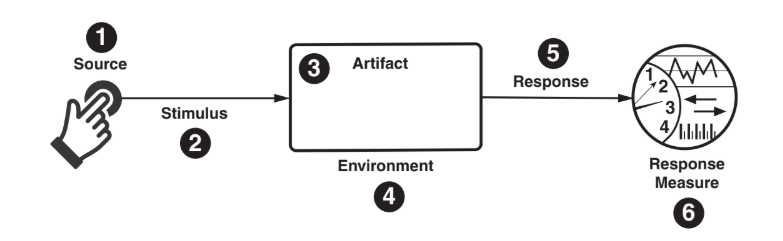
\includegraphics[width=\linewidth]{images/qa_scenario.png}
  \caption{Quality attribute scenario template}
  \caption*{Source: Software Architecture in Practice, 4th edition \cite{bass2021software}}
  \label{fig:qa_scenario_template}
\end{figure}

According to our requirements described in section \ref{sec:problem}, the two main QAs in focus are Availability and Integrability.

\subsection{Availability scenario 1}

\subsubsection{Source}
HMI is running

\subsubsection{Stimulus}
HMI crashes due to a runtime error

\subsubsection{Artifact}
HMI software

\subsubsection{Environment}
Normal operation

\subsubsection{Response}
HMI software is automatically restarted

\subsubsection{Response Measure}
Maximum downtime is 1 second

\begin{figure}[ht]
\centering
  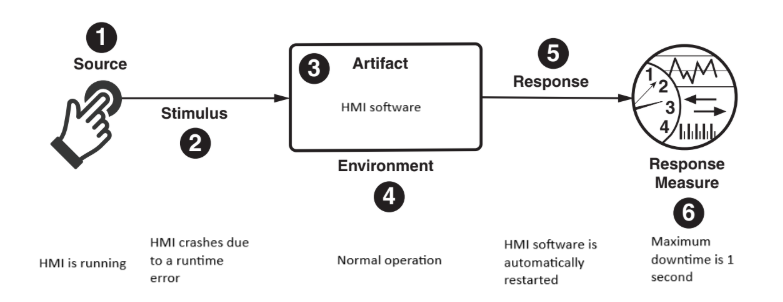
\includegraphics[height=3cm]{images/qa_scenario_hmi_downtime.png}
  \caption{Availability scenario 1}
  \caption*{Source: Software Architecture in Practice, 4th edition \cite{bass2021software}}
  \label{fig:qa_availability_scenario_1}
\end{figure}

\subsection{Availability scenario 2}

\subsubsection{Source}
Production line is running with multiple AGC instances as replicas

\subsubsection{Stimulus}
One of the AGC instances crashes

\subsubsection{Artifact}
AGC software

\subsubsection{Environment}
Normal operation

\subsubsection{Response}
The remaining AGCs continue working

\subsubsection{Response Measure}
No downtime

\begin{figure}[ht]
\centering
  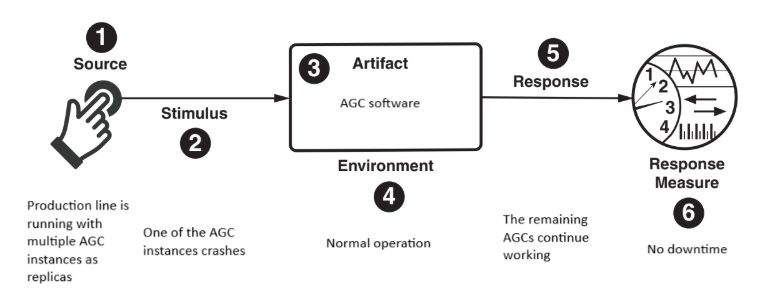
\includegraphics[height=3cm]{images/qa_scenario_agc_downtime.png}
  \caption{Availability scenario 2}
  \caption*{Source: Software Architecture in Practice, 4th edition \cite{bass2021software}}
  \label{fig:qa_availability_scenario_2}
\end{figure}

\subsection{Integrability scenario 1}

\subsubsection{Source}
Production line

\subsubsection{Stimulus}
New AGC instance is ready to add to the production line

\subsubsection{Artifact}
System

\subsubsection{Environment}
Production

\subsubsection{Response}
The new AGC is added and ready to use

\subsubsection{Response Measure}
Maximum 24 hours with no more than 24 person hours of effort
\begin{figure}[ht]
\centering
  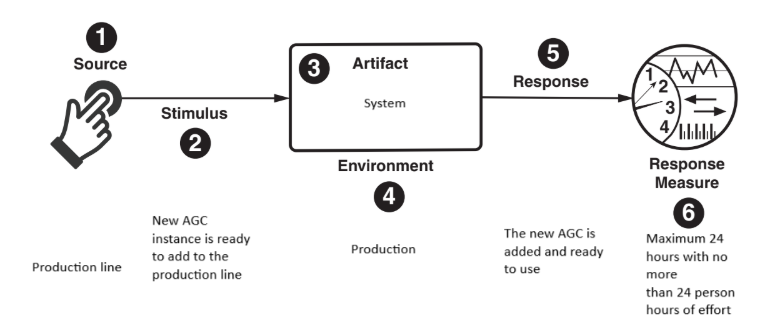
\includegraphics[height=3cm]{images/qa_scenario_deploy_new_agc.png}
  \caption{Integrability scenario 1}
  \caption*{Source: Software Architecture in Practice, 4th edition \cite{bass2021software}}
  \label{fig:qa_integrability_scenario_1}
\end{figure}

% Description of the overall architecture designs
% Argue for tactics used to archieve the QASes
% Discuss the trade-offs

%The architecture needs to support some important scenarios. The production software must run 24/7 which means that production should be able to start at any time. The production line is expected to run 7 hours a day 5 days a week on average and the product can be changed at any time, even multiple times a day. In addition to these, since the company expects a huge growth in a short period of time, the architecture should be designed in a way that new components may easily be added to the production line. Regarding these scenarios, the two main QAs in focus are Availability and Integrability.
